\documentclass[12pt]{article}
%\usepackage[utf8]{inputenc}
%\documentclass[UTF8]{ctexart}
%\usepackage[UTF8, heading = false, scheme = plain]{ctex}
\usepackage{geometry}
%geometry{a4paper,scale=0.9}
\geometry{a4paper,left=1cm,right=1cm,top=1cm,bottom=2cm}
\usepackage{amsfonts}
\usepackage{color}
\usepackage{url}
%\usepackage{biblatex}
\usepackage{amsmath}
\usepackage{amssymb}
\usepackage{latexsym}
\usepackage{cite}
%\addbibresource{ref.bib}
%\bibliography{ref.bib}
\usepackage{caption}
\usepackage{graphicx, subfig}
\usepackage{float}
%\usepackage[fontset=ubuntu]{ctex}
%\usepackage{fontspec}
\usepackage{xeCJK}
%\usepackage[colorlinks,
%anchorcolor=black,
%citecolor=black]{hyperref}
%\setmainfont{SimSun}
\usepackage[section]{placeins}
\usepackage{enumitem}
\usepackage{framed}
\usepackage[framemethod=TikZ]{mdframed}
\usepackage{indentfirst}
\usepackage{setspace}%使用间距宏包
\linespread{1.5}

\title{抽象代数的脉络\cite{Introduction_Of_Algebra_Structure}}
\author{leolinuxer}
%\date{June 2020}

\begin{document}
%\setlength{\parindent}{0pt}
\maketitle
\tableofcontents

\section{抽象代数}
\subsection{相关概念}
\subsubsection{算术(arithmetic)}
算术研究数的性质及其运算。算术运算不仅仅指加减乘除,还可以是百分比、平方根、取幂和对数;算法的对象包括自然数、整数、有理数和实数(兴许还包括复数);进制不仅仅是十进制,还可以是二进制、十六进制、六十进制。个人认为,算术的最大特点是关注具体数字。

\subsubsection{初等代数(elementary algebra)和高等代数}
用符号(成了变量)代替具体的数字,就可以得到更一般化(generalization)的等式,举例如下:
\begin{align*}
(2+3)^2 &= 2^2 + 2\times2\times3 + 3^2 \\
(3+5)^2 &= 3^2 + 2\times3\times5 + 5^2 \\
& \Rightarrow \\
(a+b)^2 &= a^2 + 2\times a \times b + b^2 \\
\end{align*}

初等代数(elementary algebra)是古老算术的推广与发展。在古代,算术积累了大量数量问题的解法,为寻求更系统、更普遍的求解各种数量关系方法,就产生了以解方程为中心的初等代数。从实际问题的数量关系(即代数式:整式、分式、根式)、等量关系(或者不等式)列出列出方程或者方程组。方程(组)包括一元/二元一次方程(linear equations with one/two variable)、一元二次方程(quadratic equations)、指数和对数方程(exponential and logarithmic equations)、无理方程(radical equations)、线性方程组(system of linear equations)。

高等代数相对于初等代数而言,本质上是一个东西,只是更加系统(深度+广度)。

\subsubsection{抽象代数(abstract algebra)}
初等代数再进一步推广(generalization),那就是抽象代数了。抽象代数(abstract algebra)、近世代数、现代代数(modern algebra)指的都是同一个意思(甚至直接称为代数学)。抽象代数主要研究对象是代数结构,包括群、环、域、向量空间。

\subsubsection{线性代数}
线性代数是抽象代数特殊的一类,其代数结构为:向量空间(vector spaces,也叫线性空间) + 线性变换(linear mappings)。很容易将线性代数和矩阵理论等同起来,但其实是不一样的,讨论\textcolor{red}{线性变换是基于选定一组基的前提下}。摘抄mathoverflow上的一个回答(原文在(\url{http://mathoverflow.net/questions/11669/what-is-the-difference-between-matrix-theory-and-linear-algebra})):

\begin{framed}
线性代数和矩阵理论的区别:

矩阵允许讨论第$i$行第$j$列的元素;

线性代数讨论的是线性变换,线性变换不是一堆数构成的矩阵,只是用矩阵来表示线性变换比较方便而已;线性代数需要给定一组基,所以讨论对应矩阵的第$i$行第$j$列的元素是不被允许的;只允许讨论不基于基的概念,比如秩、迹、行列式、特征值集合等。

来源于:http://mathoverflow.net/questions/11669/what-is-the-difference-between-matrix-theory-and-linear-algebra
\end{framed}

\subsection{代数结构(algebraic structure)}
抽象代数研究对象是代数结构,转载如下:

\begin{framed}
代数主要研究的是运算规则。一门代数, 其实都是从某种具体的运算体系中抽象出一些基本规则,建立一个公理体系,然后在这基础上进行研究。一个集合再加上一套运算规则,就构成一个代数结构(想想计算机的数据结构:数据+操作)。

来源于:http://sparkandshine.net/mit-mathematical-formalism/
\end{framed}

\subsection{初等代数$\rightarrow$抽象代数}
抽象代数将初等代数的一些概念延伸:
\begin{enumerate}[itemindent=0.5em]
\setlength{\itemsep}{0pt}
\setlength{\parsep}{0pt}
\setlength{\parskip}{0pt}
	\item 数 –> 集合
	
	\item “+ ”–> 二元运算
	
	加号“+”被抽象为二元运算 *(binary operation),\textbf{对两个元素作二元运算,得到的新元素仍然属于该集合,这叫封闭性(closure)}。实际上,加减乘除都叫二元运算(二元指的是两个操作数)。
	
	\item 0/1 –> 单位元
	
	0和1被抽象成单位元(identity elements),0为加法单位元,1为乘法单位元。单位元是集合的一个特殊元素(跟二元运算有关),满足单位元与其他元素相结合时,不改变该元素,即满足$a ∗ e = a $与$e ∗ a = a$。可见,单位元取决于元素与二元运算,如矩阵的加法单位元是零矩阵,矩阵的乘法单位元是单位矩阵。值得注意的是,有些集合不存在单位元,如正整数集合没有加法单位元
	
	\item 负数 –> 逆元素
	
	负数推广到逆元素(inverse element),对于加法,a的逆元素是-a;对于乘法,a的逆元素是倒数a−1。直观地说,逆元可以撤销操作,如加了一个数a,再加上该数的逆元-a(相当于撤消操作),结果还是一样。
	
	\item 结合律(Associative property)
	
	结合律是某些二元运算的性质,有些二元运算没有结合律(如减法、除法、八元数)
	
	\item 交换律(Commutative property)
	
	交换律,改变二元运算符两边的元素不影响结果。并不是所有二次元运算都满足交换律(如矩阵的乘法)。
\end{enumerate}

\section{Group-like}
代数结构(R, *),二元运算根据封闭性、单位元、逆元、结合律、交换律,可以归纳成不同的群。本节介绍的group-like,从最不严格到严格(依次添加限制条件),其关系图如下:
\begin{figure}[H]
    \centering
    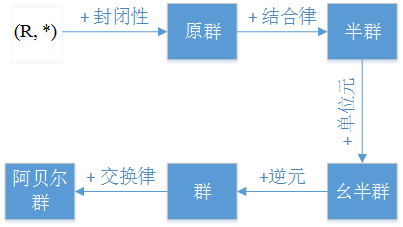
\includegraphics[width=0.5\textwidth]{fig/GroupLikeRelations.png}
\end{figure}

\subsection{原群(magma)}
原群(magma)是一种基本的代数结构,只要满足两元素作二元运算得到新元素仍属于该集合,即封闭性。

\subsection{半群(magma)}
半群(Semigroup),满足结合律(associative property)的代数结构。$V=<S,* >$,其中二元运算*是可结合的,即$(a*b)*c=a*(b*c)$,则称$V$是半群。

\subsection{幺半群(monoid)}
幺半群在半群的基础上,还需要满足有一个单位元。

\subsection{群(group)}
群(group)是两个元素作二元运算得到的一个新元素,需要满足群公理(group axioms),即:
\begin{itemize}
\setlength{\itemsep}{0pt}
\setlength{\parsep}{0pt}
\setlength{\parskip}{0pt}
\item 封闭性:$a ∗ b$仍然属于该集合
\item 结合律:$(a ∗ b) ∗ c = a ∗ (b ∗ c)$
\item 单位元:$a ∗ e = a  e ∗ a = a$
\item 逆元:加法的逆元为$-a$,乘法的逆元为倒数$1/a$,… (对于所有元素)
\end{itemize}

如整数集合,二次元运算为加法就是一个群(封闭性是显然的,加法满足结合律,单位元为0,逆元取相反数-a)。

\subsection{阿贝尔群(交换群)(Abelian Group)}
阿贝尔群在群的基础上,还需满足交换律。如整数集合和加法运算,$(Z,+)$,是一个阿贝尔群。即:
\begin{itemize}
\setlength{\itemsep}{0pt}
\setlength{\parsep}{0pt}
\setlength{\parskip}{0pt}
\item 群公理
\item 逆元:加法的逆元为$-a$,乘法的逆元为倒数$1/a$,… (对于所有元素)
\end{itemize}

\section{环论}
环在交换群基础上,进一步限制条件。环、交换环、域间的关系如下:
\begin{figure}[H]
    \centering
    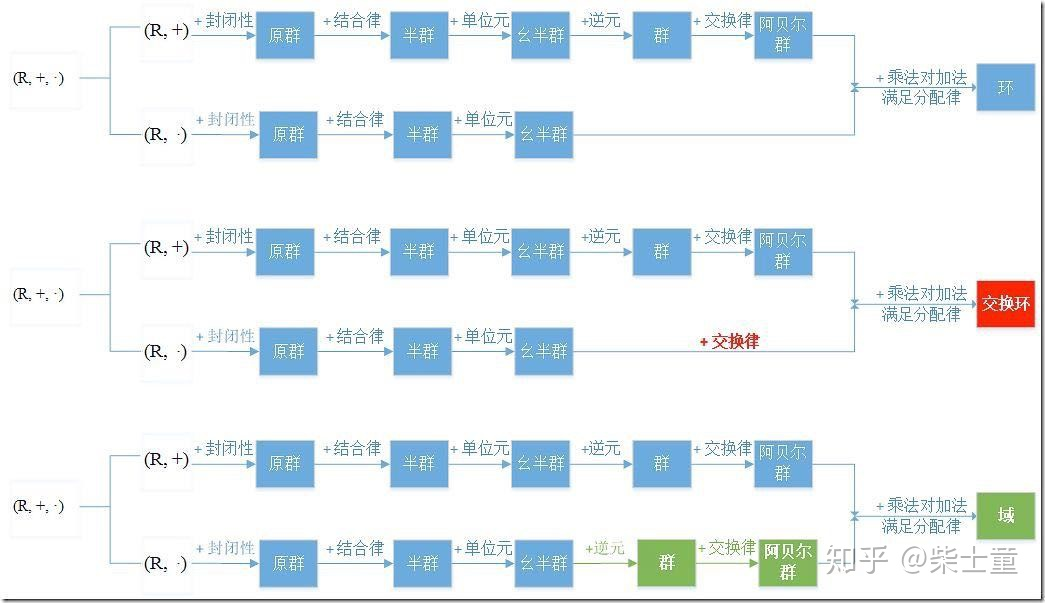
\includegraphics[width=1.0\textwidth]{fig/GroupRingField.jpg}
\end{figure}

\subsection{环(ring)}
环在阿贝尔群(也叫交换群)的基础上,添加一种二元运算·(虽叫乘法,但不同于初等代数的乘法)。一个代数结构是环$(R, +, ·)$,需要满足环公理(ring axioms)。环公理如下:
\begin{enumerate}
\setlength{\itemsep}{0pt}
\setlength{\parsep}{0pt}
\setlength{\parskip}{0pt}
\item $(R, +)$是交换群
	\begin{itemize}
	\setlength{\itemsep}{0pt}
	\setlength{\parsep}{0pt}
	\setlength{\parskip}{0pt}
	\item 封闭性:$a ∗ b$仍然属于该集合
	\item 结合律:$(a ∗ b) ∗ c = a ∗ (b ∗ c)$
	\item 单位元:$a ∗ e = a   \ \& \  e ∗ a = a$
	\item 逆元:加法的逆元为$-a$,乘法的逆元为倒数$1/a$,… (对于所有元素)
	\item 交换律:a + b = b + a
	\end{itemize}

\item $(R, ·)$是幺半群
	\begin{itemize}
	\setlength{\itemsep}{0pt}
	\setlength{\parsep}{0pt}
	\setlength{\parskip}{0pt}
	\item 结合律:$(a ⋅ b) ⋅ c = a ⋅ (b ⋅ c)$
	\item 单位元:乘法的单位元为1,$a * 1 = a   \ \& \  1 * a = a$
	\end{itemize}
	
\item 乘法对加法满足分配律
	\begin{itemize}
	\setlength{\itemsep}{0pt}
	\setlength{\parsep}{0pt}
	\setlength{\parskip}{0pt}
	\item $a ⋅ (b + c) = (a ⋅ b) + (a ⋅ c) \ \forall a, b, c \in R$
	\item $(b + c) ⋅ a = (b ⋅ a) + (c ⋅ a) \ \forall a, b, c \in R $
	\end{itemize}
\end{enumerate}

\subsection{交换环(commutative ring)}
交换环(commutative ring)在环的基础上,二元运算乘法还满足交换律。

\subsection{整环(integral domain)}
整环在交换环的基础上,并满足没有零因子(如此,集合内任意两个元素乘积均不等于0)

\section{域(Field)}
域(Field)在交换环的基础上,还增加了二元运算除法,要求元素(除零以外)可以作除法运算,即每个非零的元素都要有乘法逆元。由此可见,\textbf{域是一种可以进行加减乘除(除0以外)的代数结构,是数域与四则运算的推广}。整数集合,不存在乘法逆元(1/3不是整数),所以整数集合不是域;有理数、实数、复数可以形成域,分别叫有理数域、实数域、复数域。

\section{向量空间(vector space)}
向量空间是一些向量的集合。最熟悉的例子是几何向量或矢量(Euclidean vectors, geometric vector, spatial vector),表示具有大小和方向的对象;矢量可以做加法(addition)和乘法(scalar multiplication)运算

其他例子,还包括坐标空间(Coordinate spaces)、复数、函数空间(Function spaces)、线性方程组(linear equations)。

\subsection{8个公理}
给定域F,向量空间V记为F-向量空间。其二元运算:
\begin{itemize}
\setlength{\itemsep}{0pt}
\setlength{\parsep}{0pt}
\setlength{\parskip}{0pt}
\item 向量加法:$+ : V × V → V$ 记作 $v + w, \exists v, w \in V$
\item 标量乘法:$·: F × V → V$ 记作 $a \cdot v, \exists a \in F, v \in V$
\end{itemize}

并且满足如下8条公理:
\begin{itemize}
\setlength{\itemsep}{0pt}
\setlength{\parsep}{0pt}
\setlength{\parskip}{0pt}
\item 向量加法结合律:$u + (v + w) = (u + v) + w$
\item 向量加法的单位元:V存在零向量的0,$\forall v \in V , v + 0 = v$
\item 向量加法的逆元素:$\forall v \in V, \exists w \in V$,使得 $v + w = 0$
\item 向量加法交换律:$v + w = w + v$
\item 标量乘法与域乘法兼容性(compatibility): $a(b v) = (ab)v$
\item 标量乘法有单位元: $1 v = v$, 1指域F的乘法单位元
\item 标量乘法对于向量加法满足分配律:$a(v + w) = a v + a w$
\item 标量乘法对于域加法满足分配律: $(a + b)v = a v + b v$
\end{itemize}

另,若F是实数域$\mathbb{R}$,则V称为实数向量空间;若F是复数域$\mathbb{C}$,则V称为复数向量空间;若F是有限域,则V称为有限域向量空间。

\section{模(module)}
模是对向量空间的推广,将标量需为域(向量空间)推广到任意环(模)。

\section{代数(algebra)(环论)}
代数将algebra over a field中的域推广到交换环。

\section{格(lattice)}
格是任意两个元素都有上确界和下确界的偏序集合。

\section{总结}
是时候,祭出这张图了,图片来源于(\url{http://mccabism.blogspot.fr/2007_03_01_archive.html})
\begin{figure}[H]
    \centering
    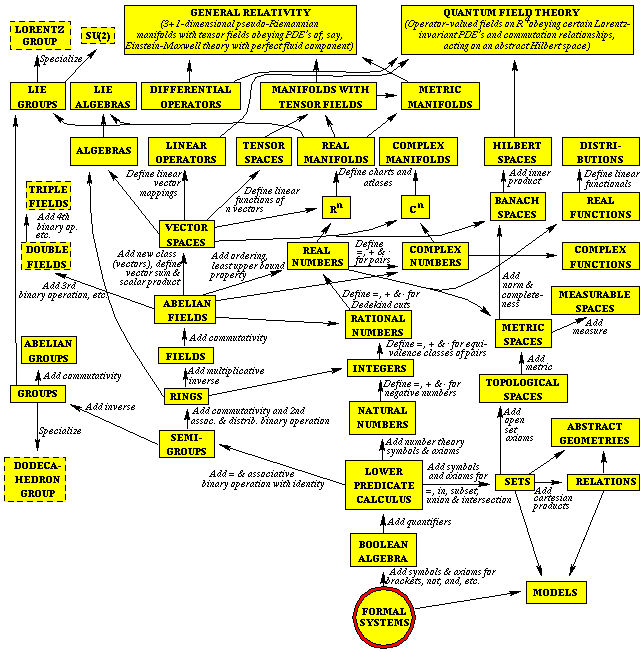
\includegraphics[width=1.0\textwidth]{fig/AbstractAlgebraRelations.png}
\end{figure}

%\printbibliography
\bibliography{../ref}
\bibliographystyle{IEEEtran}
\end{document}
